\documentclass[conference]{IEEEtran}
\IEEEoverridecommandlockouts
% The preceding line is only needed to identify funding in the first footnote. If that is unneeded, please comment it out.
\usepackage{cite}
\usepackage{amsmath,amssymb,amsfonts}
\usepackage{algorithmic}
\usepackage{graphicx}
\usepackage{textcomp}
\usepackage{xcolor}
\def\BibTeX{{\rm B\kern-.05em{\sc i\kern-.025em b}\kern-.08em
    T\kern-.1667em\lower.7ex\hbox{E}\kern-.125emX}}
\begin{document}

\title{Brain ViT: Multi-Label Classification of Brain Pathologies using Vision Transformers \\
}

\author{\IEEEauthorblockN{Sony Reddy Gurram}
\IEEEauthorblockA{\textit{University of South Dakota} \\
Vermillion, SD\\
SonyReddy.Gurram@coyotes.usd.edu}
\and
\IEEEauthorblockN{Sainath Vaddi}
\IEEEauthorblockA{\textit{University of South Dakota} \\
Vermillion, SD\\
Sainath.Vaddi@coyotes.usd.edu}
\and
\IEEEauthorblockN{Neerajdattu Dattum}
\IEEEauthorblockA{\textit{University of South Dakota} \\
Vermillion, SD \\
Neerajdattu.Dattum@coyotes.usd.edu}
\and
\IEEEauthorblockN{Drake Michael Farrokhi}
\IEEEauthorblockA{\textit{University of South Dakota} \\
Vermillion, SD \\
Drake.Farrokhi@coyotes.usd.edu}
\and
\IEEEauthorblockN{Dr. Rodrigue Rizk}
\IEEEauthorblockA{\textit{University of South Dakota} \\
Vermillion, SD \\
Rodrigue.Rizk@usd.edu}
\and
\IEEEauthorblockN{Dr. K.C. Santosh}
\IEEEauthorblockA{\textit{University of South Dakota} \\
Vermillion, SD \\
KC.Santosh@usd.edu}
}

\maketitle

\begin{abstract}
After the invention of the transformer model in 2017 and the related advancements in language processing, researchers have been highly interested in the adaptability of the transformer architecture. Recent days, transformers are highly used to perform computer vision tasks. Based on the same intuition, we propose Brain ViT, a Vision Transformer-based model for identifying brain pathologies. The model can classify MRI scans between multiple categories: no brain tumor and brain tumor which include glioma, meningioma, and pituitary.

\end{abstract}

\begin{IEEEkeywords}
Machine Learning, Neural Network, Vision Transformer
\end{IEEEkeywords}

\section{Introduction}
The advent of the transformer model architecture by Vaswani et. al. in their 2017 paper \textit{Attention is All you need}$^1$, along with the corresponding success seen in its application to natural language processing (NLP) tasks.  This revolutionized NLP tasks such as machine translation, text summarizing, and language understanding, which has led to the architecture being applied to other tasks. This intern led to the invention of a model architecture, quite similar in nature to the original transformer models, dubbed Vision Transformers (ViTs). The transformers self-attention mechanism enables the capture of long-range dependencies within sequential data as well as short-range dependencies which proves to be highly valuable in the computer vision realm.

Motivated by this trend and the corresponding success seen with ViTs in computer vision tasks, we introduce BrainViT, a novel ViT model tailored for the classification of brain pathologies from magnetic resonance imagery (MRI) scans. The application of deep learning techniques to medical imagery data has seen astonishing success in recent years promising the potential for more accurate and efficient diagnosis and treatment planning for patients. However, challenges remain due to the rich spatial information and structural information present in this type of data.

BrainViT aims to tackle these challenges via the nature of the self-attention mechanism to capture the intricate patterns and relationships found within MRI data. Specifically, our model is designed and trained to classify MRI scans into four distinct categories: glioma, menigioma, or pituitary tumors along with the absence of any untrained tumor type or potentially healthy brain MRI. BrainViT offers a promising approach to enhancing and increasing the accuracy and reliability and decreasing the time required for receiving a diagnosis which leads to improved patient care and clinical outcomes. 

In this paper, we present a detailed description of the BrainViT architecture. We then evaluate the model on balanced testing datasets demonstrating its effectiveness in accurately classifying brain pathologies. Additionally, we discuss BrainViT's advantages over existing diangosis methodologies along with potential avenues of future research and the broader implications of BrainViT within the field of medical imagery analysis and computer-aided diagnosis.

\section{Ease of Use}

BrainViT is quite easy to use from a medical practitioners point of view - once the MRI image has been loaded into the model, BrainViT will accurately classify the image with the assumption that the tumor type is within the trained pathology list. Furthermore, given a large enough dataset and access to high performance computing, BrainViT can quickly be trained to identify other brain pathologies. For access to the pretrained BrainViT model navigate to https://github.com/vivekkiran/BrainViT.

BrainViT also provides medical practitioners a highly reliable, quick, and accurate diagnosis methodology. Typically, to make a diagnosis, one would have to have multiple tests run such as imaging, biopsies, and blood tests, all of which would have to be interpreted by someone how has gone through many years of schooling and training to be able to make a confident diagnosis. Comparing this to BrainViT which trained in under one month on a relatively small dataset, BrainViT is the clear victor and will see higher accuracy and confidence in diagnosis with larger datasets and longer training times.

\section{Materials and Methods}
BrainViT results were gathered by using the publicly available dataset Brain Tumor MRI Dataset from kaggle$^2$. BrainViT was produced by using a pretrained ViT model called ViT B16 produced by Google which is publicly available from pytorch's torchvision transformers module$^3$.

The MRI dataset consists of four distinct classes which are glioma, meningioma, and pituitary tumors along with a class for absence of tumors. The images found within the dataset are gathered from three different datasets: the figshare dataset$^4$, the SARTAJ dataset$^5$, and the Br35H dataset$^6$. The dataset is presplit into training and testing categories with a 80/20 training/testing split (N$_{training}$ = 5712, N$_{testing}$ = 1311). Finally, the dataset is well-balanced with a difference of 274 data points within the training set and 105 data points within the testing set. 

The pretrained B16 ViT model produced by Google is a rather typical ViT. The B16 ViT model takes in a flattened or linear positionally-embedded patched image that gets fed through a multi-head attention layer initially then into two fully connected layers and finally into a mutli-layer perceptron (MLP) head that performs the classification. Furthermore, there are residual connections between the input layer and the output of the multi-head attention layer as well as from the output of the multi-head attention layer to the input of the MLP.

Rather than update the size of the input layer, we rescaled our images to 224x224 as is standard practice with this model. Furthermore, we employed the Adam optimizer along with a loss function of cross entropy at a learning rate of 1e$^{-3}$ and we set the torch and torch.cuda random seed value to 42. The pretrained B16 ViT also expects three color channels; however, given that our MRI images are in grey scale, we adjusted the model's input layer to accept one color channel. Finally, we froze the model in all layers except in the MLP to fine tune classification.

\begin{figure}[h]
    \centering
    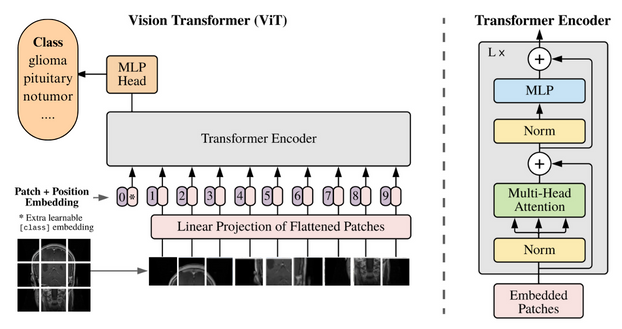
\includegraphics[width=0.45\textwidth]{arch.png}
    \caption{BrainViT Architecture.}
    \label{fig:graphs}
\end{figure}

\section{Results}
We trained the model for 30 epochs at which point we were observing a training accuracy of 98.64\% along with a testing accuracy of 95.20\%.

\begin{table}[h]
    \centering
    \caption{Precision, Recall, and F1 Score by Class}
    \label{tab:example_with_headers}
    \begin{tabular}{|c|c|c|c|}
        \hline
        \textbf{Class} & \textbf{Precision} & \textbf{Recall} & \textbf{F1 Score} \\ 
        \hline
        Glioma & 0.97 & 0.92 & 0.95 \\ 
        Meningioma & 0.86 & 0.98 & 0.91 \\ 
        Pituitary & 0.99 & 0.99 & 0.99 \\
        Not Tumor & 1.00 & 0.93 & 0.96 \\
        \hline
    \end{tabular}
\end{table}

\begin{figure}[h]
    \centering
    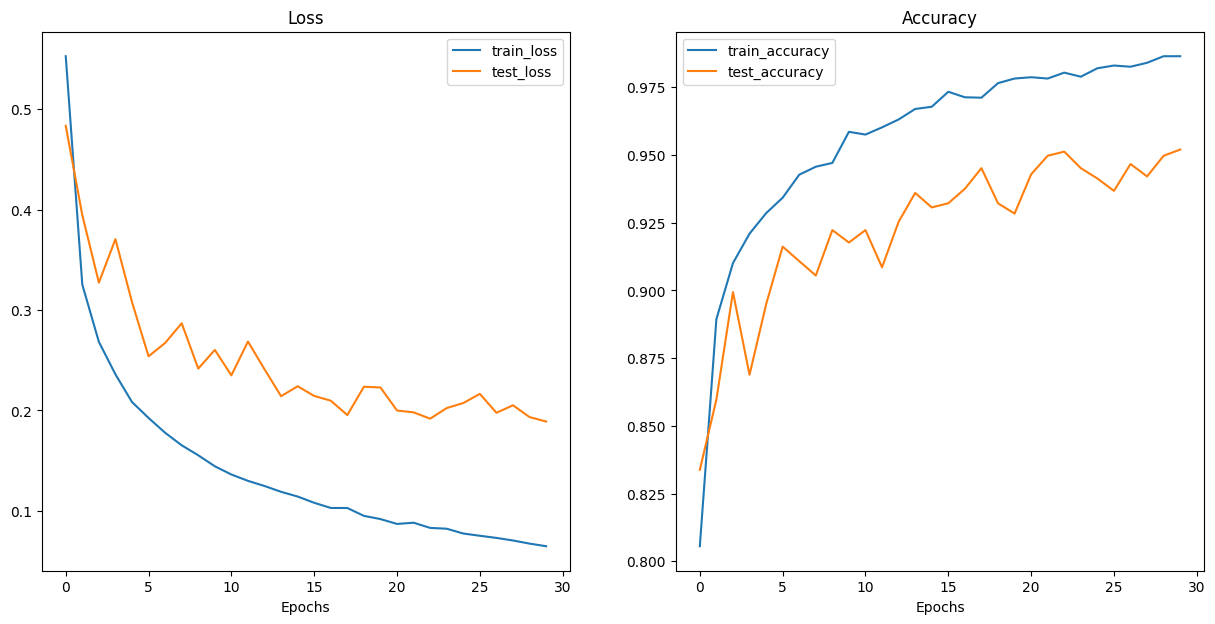
\includegraphics[width=0.45\textwidth]{graph.png}
    \caption{Plot of loss function and accuracy over 30 training epochs.}
    \label{fig:graphs}
\end{figure}

\section{Discussion}
BrainVit was able to produce high accuracy classification with a relatively small training time given how many epochs ViT models are typically trained for. With that being said, given a large dataset - to avoid overfitting - along with access to HPC, one would likely see much higher accuracy. Furthermore, given a dataset with more classes, we believe the model will likely perform well in this case as well given that the B16 ViT model has been known to be able to perform well on the ImageNet 1000 class dataset.
Having shown proof of concept, the next step will be to produce a similar ViT architecture in the Julia programming language which has seen great success, performance, and speed within the machine learning/data science field. After having produced this model we will be able to train it on a larger dataset with more classes on HPC at the University of South Dakota.

\section*{Acknowledgment}
We thank the University of South Dakota for granting us HPC access during the summer of 2024 to train our Julia BrainViT. Further thanks to Dr. Rodrgiue Rizk and Dr. K.C. Santosh for providing support and guidance during this project. Finally, we thank to the 2AI volunteer team at the University of South Dakota for collaborating and assisting with idea development and providing feedback.

\begin{thebibliography}{00}
\bibitem{b1} A. Vaswani et al., “Attention is all you need,” in Advances in Neural Information Processing Systems, 2017.
\bibitem{b2} M. Nickparvar. "Brain tumor MRI dataset," in Kaggle, 2021. 
\bibitem{b3} PyTorch, "ViT-B/16: Vision Transformer with BERT-style tokens," PyTorch torchvision Library.
\bibitem{b4} J. Cheng, "Brain tumor dataset," 2017.
\bibitem{b5} J. Sarta, "Brain tumor classification (MRI)," in Kaggle, 2020.
\bibitem{b6} A. Hamada, "Br35H:: Brain tumor detection 2021," in Kaggle, 2020.
\bibitem{b7} A. Dosovitskiy et al., “AN IMAGE IS WORTH 16X16 WORDS: TRANSFORMERS FOR IMAGE RECOGNITION AT SCALE,” in ICLR 2021 - 9th International Conference on Learning Representations, 2021.
\end{thebibliography}
\end{document}
